% Activate the following line by filling in the right side. If for example the name of the root file is Main.tex, write
% "...root = Main.tex" if the chapter file is in the same directory, and "...root = ../Main.tex" if the chapter is in a subdirectory.
 
%!TEX root =  

\chapter[Systematics]{Systematic Errors}

\section{Systematic Errors on the Signal}
\subsection{Trigger Efficiency}
\subsection{Jet Energy Scale and Resolution}
\subsection{Signal Monte Carlo Generator Systematics}

\section{Systematic Errors on the Background Estimation}
\subsection{Systematic Errors on Data-Driven Background Estimates}

\begin{figure}
    \centering
    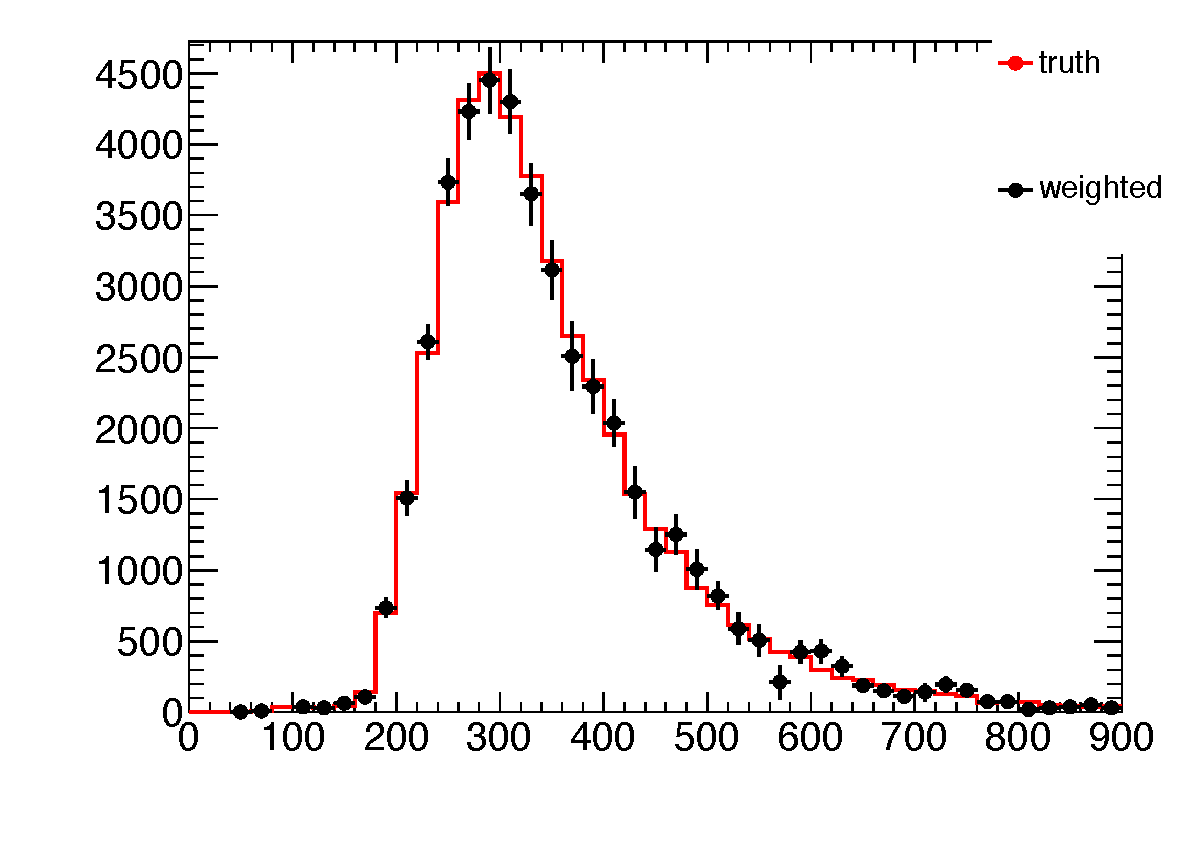
\includegraphics[width=0.3\linewidth]{/Users/caitlinmalone/Documents/Thesis/Systematics/mm_shape_check_b.pdf}
    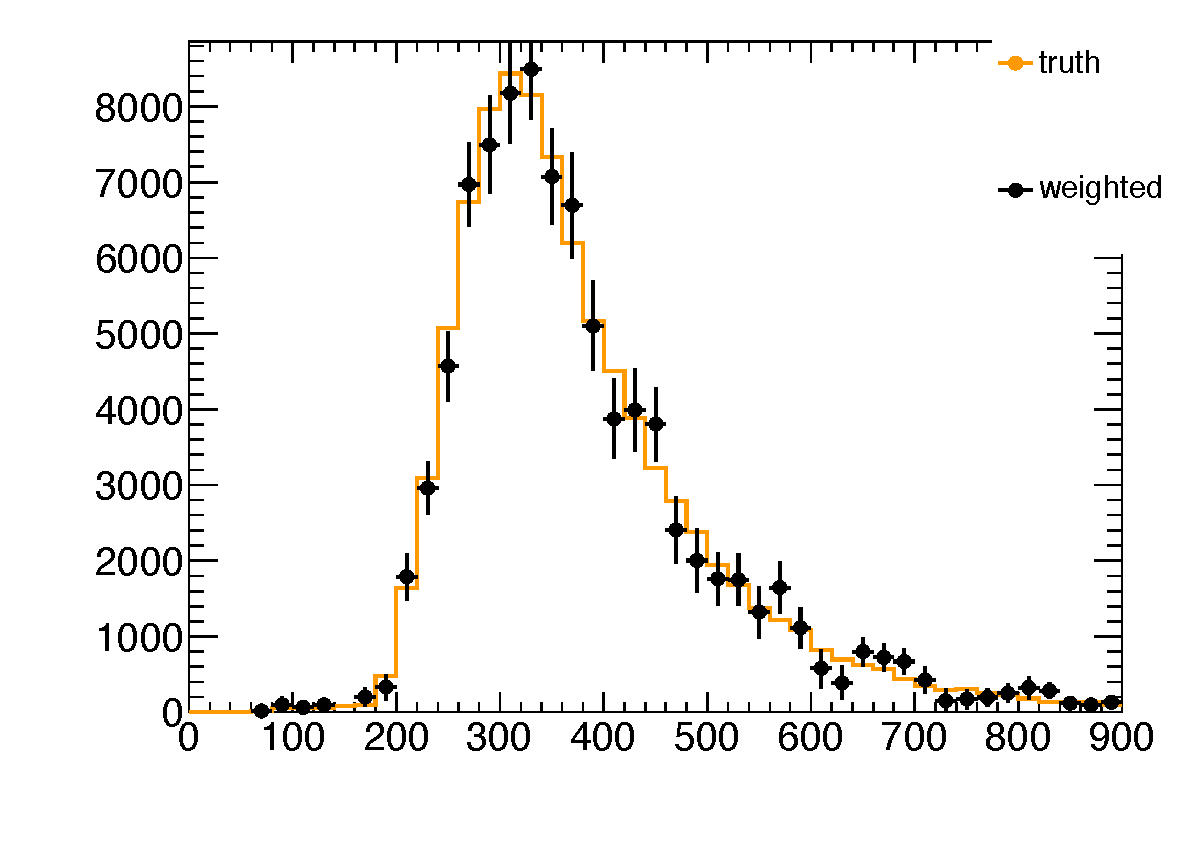
\includegraphics[width=0.3\linewidth]{/Users/caitlinmalone/Documents/Thesis/Systematics/mm_shape_check_c.pdf}
    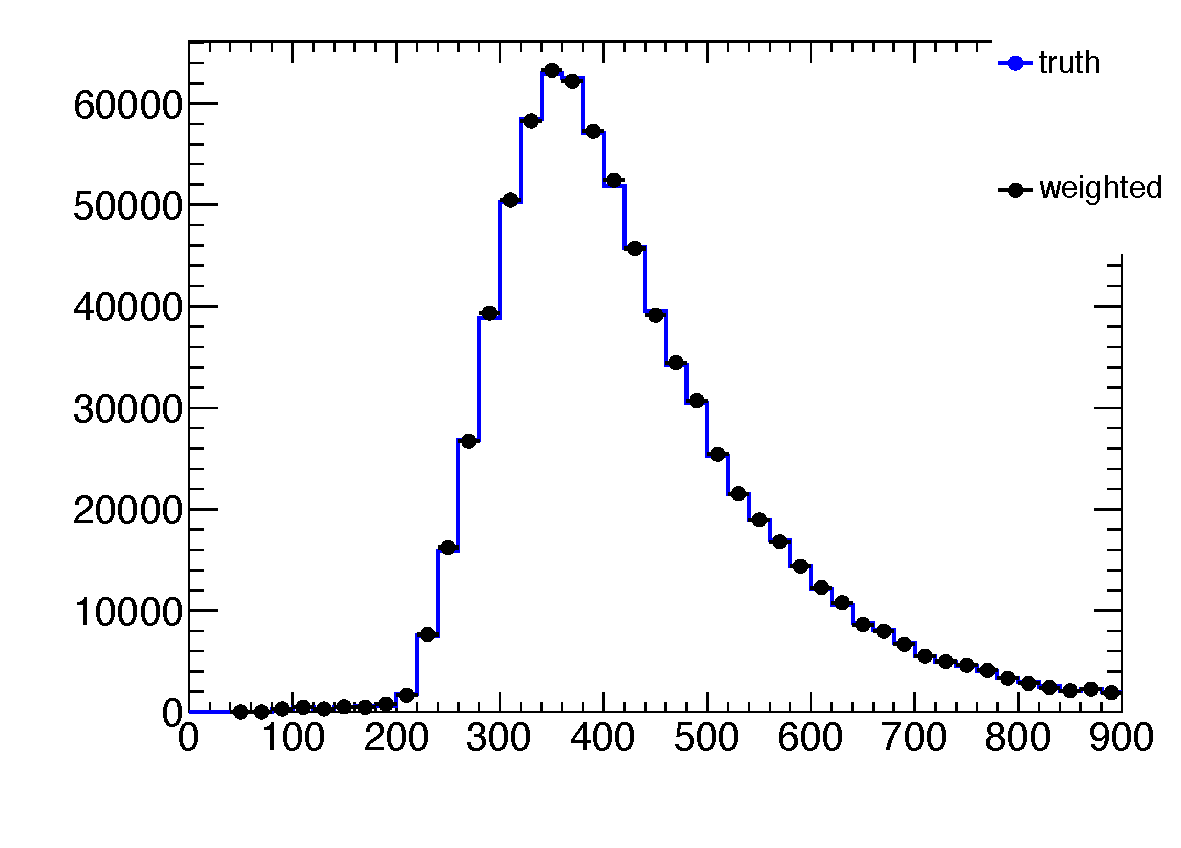
\includegraphics[width=0.3\linewidth]{/Users/caitlinmalone/Documents/Thesis/Systematics/mm_shape_check_light.pdf}
    \caption{A comparison of the toy $m_{bb}$ distributions for the different flavors of the
        third jet, as shown in Figure~\ref{fig:mbb_compare_truth_spectra}, with the matrix
        method predictions overlaid.  }
    \label{fig:mbb_compare_truth_mm_toy}
\end{figure}

\subsection{Systematic Errors on MC-Derived Background Estimates}





